\chapter{前期の主な活動}
私達大学グループは，当初病院グループとして結成された．函館市の病院に関連するサービスを作ることで，病院を利用する際の利便性を高めようとすることが目的のグループである．

\bunseki{大須賀雅也}

\section{病院グループとしての活動}

\subsection{既存のサービスの調査}
私達は，5月24日のグループワークで，函館に存在する病院関連サービスの問題点と良い点を調査した．はこだて医療情報\footnote{http://www.medical-h.net}というWebサイトとGrucco\footnote{https://www.city.hakodate.hokkaido.jp/docs/2017051700047/}というモバイルアプリを調査の対象とした．グループの全員でそれぞれのサービスに実際に触れてみた．触れた結果挙がった感想を以下に記述する．
\vskip\baselineskip

\begin{description}
\item[はこだて医療情報] \mbox{} \\\\
良いところ
\\
\begin{itemize}
\item 情報が網羅されていそう
\item 検索は意外とできそう
\item 詳しくのっていそう
\end{itemize}
\mbox{} \\
悪いところ
\\
\begin{itemize}
\item 使いにくい
\item 検索システムが見づらい
\item ダサい
\item 地図が使えない
\item 自分で入力して検索することができない
\item スマホでみにくい
\item 検索するのに時間がかかる
\item 情報が飽和していて必要な情報を選びづらい
\item 存在するはずの情報が存在しない
\item 古い
\end{itemize}

\end{description}

\clearpage
\begin{description}
\item[Grucco] \mbox{} \\\\
良いところ
\vskip\baselineskip
\begin{itemize}
\item 健診\item 予防接種のお知らせの通知設定ができる
\item 記事のお気に入り機能がある
\end{itemize}
\mbox{} \\
悪いところ
\\\\
全体
\begin{itemize}
\item 最新Androidのバージョンに対応していない
\item 定期的にフッターメニュー押せなくなる
\item アイコンが各タブで統一されている→ホームの新着情報で区別できるけど
\end{itemize}
\mbox{} \\
ホーム
\begin{itemize}
\item 夜間急病センター案内へのリンク飛ばし
\item ジャンルの順番
\item こちらから検索，検索わかりにくい
\end{itemize}
\mbox{} \\
施設
\begin{itemize}
\item ジャンルによるピンに違いがない，全部これ
\item ジャンル複数選択できない
\item 病院というジャンルが存在しない
\end{itemize}
\mbox{} \\
イベント
\begin{itemize}
\item 日付の記載が日付欄とタイトル【】でばらばら
\item お知らせ
\item お気に入り
\item 施設ページから地図をみれない
\end{itemize}

\end{description}

\bunseki{大須賀雅也}

\subsection{ペルソナ分析}
TAの方から，対象者を考える時はペルソナを用いて考える事によって，グループメンバーが対象者を想像しやすくなるというご指摘を受けたため，グループメンバーでペルソナを考えることにした．ChatGPT\footnote{https://chat.openai.com/}を用いて，10代から80代までの存在しない人物のプロフィールを生成し，それぞれの人物が「どのような時に病院を利用するか」「なぜ病院を探すのか」について検討した．

\bunseki{大須賀雅也}

\section{テーマの変更}
%1.3節で述べた課題をより具体的に記述する．成果に対して必ず満たすべき条件を含む

私達は，5月31日に行ったグループワークで，それまでに検討していた病院に関連したアプリのアイディアに行き詰まり，次回までの宿題として「アプリを作る前提でのコンセプト」「方向性，機能」などをそれぞれ各自で考えてくることとした．そして，6月2日のグループワークで，それぞれの考えてきたことを発表しあった．その結果，自分たちが在籍している公立はこだて未来大学に関連するアプリを開発するという案が採用された．採用された理由は，公立はこだて未来大学は私達が在籍している大学であるため，存在する問題を詳しく理解している．加えて，存在する問題を解決することが私たちに直接役に立つため，以前の病院に関連したアプリ開発よりモチベーションが維持しやすいからである．


\bunseki{大須賀雅也}

\section{公立はこだて未来大学の問題点}
次に，公立はこだて未来大学に存在する問題について具体的に考えた．真っ先に挙げられた問題は，公立はこだて未来大学のシステムが使いにくいということであった．具体的には，「HOPE\footnote{https://hope.fun.ac.jp/}やSTUDENTS\footnote{https://students.fun.ac.jp}のどこにどの情報があるのかがわからない」や「情報がまとまっていない」などである．そしてHOPEやSTUDENTSのどういった情報が必要なのかを検討した．私たちが必要だと感じた情報として以下の様な案が挙げられた.
\begin{itemize}
      \item 単位にかかわる詳細情報
      \item 評価基準
      \item 授業フィードバック
      \item 課題に関する情報
      \item 先生方のメールアドレス
      \item 教室情報
\end{itemize}
これらの情報は，HOPEやSTUDENTSに存在するが探すのが面倒であったり，そもそもどこにあるかがわからないという問題があることが分かった．そのため，これらの情報をまとめるということが一つの課題となった．

\bunseki{大須賀雅也}

\section{プロダクトの考案}
次に，大学で生活するうえでどんなサービスが欲しいかについて意見を出し合いホワイトボードにアイディアを羅列していった．そこで，「学生間で不必要になったものなどをやり取りするもの（ジモティのようなもの）」「学内，学外アルバイト」「飲食店の情報」「料理の情報」「過去問」「テーブルの空きがわかるマップ」「課題の締め切り情報一覧」などの意見が出た．そして，ここまでで出たアイディアの中でどのサービスが一番欲しいかグループ内で投票をした．その結果「学生間で不必要になったものなどをやり取りするもの（ジモティのようなもの）」「過去問」「課題情報」「テーブルの空きがわかるマップ」が私たちが欲しているものだということが分かった．そこで，以下の四つの軸でアプリを開発することに決定した．
\begin{itemize}
      \item 情報系
      \item 学生間で不必要になったものなどをやり取りするもの（ジモティのようなもの）
      \item 授業系
      \item マップ系
\end{itemize}
そして，この四つの軸にどのような機能を実装するかホワイトボードに書き出してまとめる作業を行った．情報系は「バイト」「イベント」「過去問」「就活」などの情報を表示する．授業系は「課題締め切り」「授業フィードバック」「VEP関連」「単位情報」「評価基準」などの情報をまとめる．マップ系は「テーブルの空き」「教室の空き」「コンセントの場所」「部屋の名称」「気温や空調」などを表示する．「学生間で不必要になったものなどをやり取りするもの（ジモティのようなもの）」は教科書や家具や服や備品などをやり取りできるようにする．

\bunseki{大須賀雅也}

\section{ブレインストーミング}

ブレインストーミングはホワイトボードを使って行った（図\ref{fig:brain}）．グループのメンバーがそれぞれ思いついたアイディアを書いていくという形をとった．ブレインストーミングでは公立はこだて未来大学の問題だけではなく，あったらいいものや欲しいものなど様々なアイディアが挙げられた．ブレインストーミングにはTAの方にも協力していただき様々なアイディアやアドバイスを頂いた．
\begin{figure}[H]
    \centering
    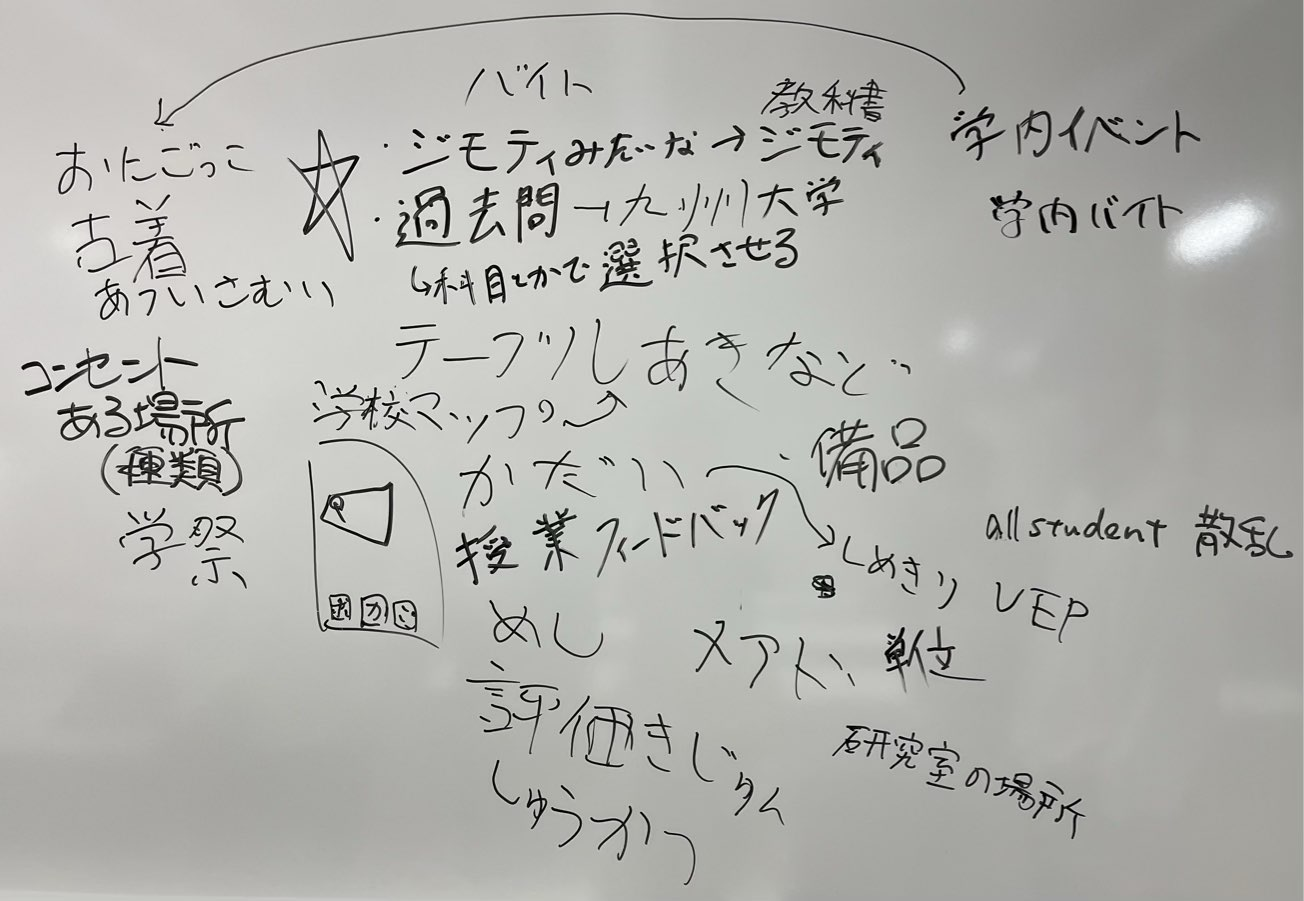
\includegraphics[width=8cm]{images/2.2_whiteboard.jpg}
    \caption{ホワイトボードの板書}
    \figlab{brain}
\end{figure}

\bunseki{大須賀雅也}

\section{フィールドワーク}

学内での問題点をより明白化するために，すでに自分たちで推測した問題点を意識して大学内を歩き回った．空き教室や空きテーブルをわざわざ歩いて探す必要があったり，コンセントも実際に行かないとあるか分からないのが現状だった．また，情報集めの一環として周りの友人に話を聞いた．大学に対する不満や問題点，現在検討中のアイディアへの意見，どんな機能があったら良いかなどを質問した．検討中のアイディアとしては，空きテーブルの情報，教科書などを受け渡すコミュニティや情報をまとめるなどがある．学生の不満点として共通していたのは，情報の集めづらさであった．HOPEやSTUDENTSといった各サイトに情報が散らばっていたり，書いている情報が違っているという状況に困惑している学生が多かった．また，検討中のアイディアに対して，絶対に必要な機能というわけではないが，あればとても便利になるという意見が多く，公立はこだて未来大学の問題点を再認識することができた．

\bunseki{齊藤輝}


\section{プロダクトの決定}

6月2日に公立はこだて未来大学で使えるアプリという案の問題点と新たなプロダクト案に関するブレインストーミングを行った．授業の課題などの科目情報，その他の学校に関することなど分散した情報を統合したいと話し合ったが，情報を取得する技術をどうするかが議題となった．科目によって課題の公開の仕方は別々であるため，API取得といった技術を使用する必要があるが，現状可能なのか分からなかったため，卒業研究で同じ分野に取り組んでいる方に話を聞いた．現在オープンデータを作っていて時間がかかるため待つしかないとのことなので，他のアイディアを深掘りすることにした．TAの方が，「まずはとにかくアイディアを出したほうが良い」と仰っていた．そのため，実際にアプリで何をしたいかホワイトボードに書き出した．どのような機能があって誰が対象なのか，何を解決できるかなどを話し合った．また，そのアイディアが実現可能なのかその都度担当教員に確認しながら進めた．最終的に，空き教室なども分かる学内のマップ，過去問，科目情報やその他の情報，教科書などを受け渡すコミュニティの機能を揃えたアプリを作成することに決定した．

\bunseki{齊藤輝}

\section{既存サービスの調査}

私達は6月7日に既存のサービスがないか調査を行った．その結果，「九州大学（非公式）\footnote{https://apps.apple.com/jp/app/九州大学-非公式/id158535402}\footnote{https://play.google.com/store/apps/details?id=com.kaede.KyushuUniversity}」「東海大学　スクールアプリ\footnote{https://apps.apple.com/jp/app/東海大学-スクールアプリ/id610479211}\footnote{https://play.google.com/store/apps/details?id=jp.co.disc.schoolnavi.dhdeijj}」などがあることがわかった．これらのアプリは，学生証，大学のホームページと連携したニュース，アプリのレビュー，時間割，学校生活についての情報などの機能を有していることがわかった．既存のアプリケーションでは空き教室や空きテーブルやコンセントの位置情報を提供しているものはない．既存のアプリケーションでは自分たちが必要としている機能には対応していない．また学生同士が教科書の受け渡しをするコミュニティの提供もない．学生はキャンパス内の施設やイベント，サービスに関する情報をパソコンからではなく手元にあるモバイル端末から簡単に入手できる．また公立はこだて未来大学ではWebアプリとして，着席QRコード読み取りを便利にするスマートフォン向けアプリケーションRALAF\footnote{https://fun-dev.github.io/RALAF/}（ららふ）がリリースされており，コロナ禍における教室での着席にQRコードによる学内での入退室着座登録を行っていた．

\bunseki{高橋慧流}

\section{技術検証}

私達は6月7日に奥野教授から大学の時間割情報を取得できるAPIについての話を頂いた．さらにTAの方から6月9日にOpenDBと実装状況についての説明を頂いた．OpenDBとは公立はこだて未来大学の教務システムのデータをAPIで提供するシステムである．実際には教務システムとOpenDBのデータベースは別であり，毎日0時に教務システムのデータベースからOpenDBのデータベースにコピーするパッチが実行される．7月18日現在，OpenDBでは主に時間割情報を取得できる．時間割情報として，時間割，教室，教室変更，休講，補講があり，時間割曜時（開講される曜日時限），時間割副担当教職員，時間割教室（開講される教室）は時間割に対して複数存在するため，エンティティを分割する．時間割は時間割一覧を取得するほか，時間割コードを指定すると指定された時間割を取得できる．教室は教室一覧を取得するほか，教室コードを指定すると指定された教室を取得できる．教室変更は教室変更一覧を取得できる．休講は休講一覧を取得できる．補講は補講一覧を取得できる．時間割曜時は，時間割コードを指定するとその時間割の開講曜日と時限が複数取得できる．時間割副担当教職員は，時間割コードを指定するとその時間割の副担当教員を複数取得できる．時間割教室は，時間割コードを指定すると教室コードを複数取得できる．
\bunseki{南川虎之介}


\section{プロダクト名の決定}

プロダクトの機能が完全には決まっていないため，プロダクト名はまだ決定できていない．
\bunseki{鈴木利芳}

\section{対象者の明確化}

私達が開発するサービスの対象者は，公立はこだて未来大学に在籍している学生である．私達が対象者について考え始めたのは6月2日のグループワークである．私達はプロジェクト学習で開発するものは，私達自身に役に立つものにしたいという思いがあった．そういったサービスであれば問題の改善に対するモチベーションが高くなると考えたからである．そのため，私達全員が利用しているものを改善したいと考えた．その条件を満たしたうえで積極的に改善したいものを考えた結果が公立はこだて未来大学であった．こういった理由から公立はこだて未来大学に在籍している学生が対象者となった．
\bunseki{大須賀雅也}

\section{問題の明確化}

私達が最初に提起した問題は「大学のシステムが使いにくい」であった．これは私達が公立はこだて未来大学を対象にしたサービスを作ると決まった時，真っ先に挙げられた問題である．私達は，公立はこだて未来大学に在籍している学生として，日々大学が提供したシステムを利用している．公立はこだて未来大学のシステムがなぜ使いにくいのかについての意見を出し合った．その結果，HOPEやSTUDENTSの情報がまとまっていないということが分かった．ほかに提起された問題は，空き教室の情報がどこにあるのかわからないということである．授業と授業の間の空き時間に課題などを行うための空き教室を探すのが面倒で分かりにくいということである．それに付随して，空きテーブルを探すのも面倒だという意見も出た．
\bunseki{大須賀雅也}

\section{目的の明確化}

私達の当初のコンセプトは「痒いところにすぐ手が届く」というものであり，目的は「自分たちが使いやすいものを作る」というものであった．これは，実際に公立はこだて未来大学の学生として過ごして，情報が分散していたり，空き教室を探すことが大変であるといった問題点を自分たちで実感し，この問題をもとに決めた目的である．\par
一度この内容で中間発表用のスライドに記述したところ，奥野教授から，「作ることが目的になっていないか」というフィードバックを頂いた．このフィードバックをもとにグループメンバー全体で改めて目的として適切であるか話し合ったところ，もっと具体的な結果を含む内容にしたいという考えに至った．この目的は，何を作りたいのかも分からない曖昧な内容になってしまっていた．理想の目的は，背景となった問題点を解決することであり，その内容を含む内容にしたいと考えた．最終的には，「未来大の情報をまとめたアプリを作り利便性を高めたい」という目的に決定することにした．
\bunseki{齊藤輝}

\section{ヒアリング}

中間発表後の質疑応答の時間を利用して,アプリに欲しい機能があるか聞いた.案として,車の相乗り機能や先輩方の科目のフィードバック機能,サークル情報,院試情報などが挙げられた.

\bunseki{齊藤輝}

\section{中間発表}
\subsection{準備}
中間発表はプロジェクト間での交流を目的とし，それに向けてプロジェクトの内容を紹介するメインポスター，スライド，スピーカーノートを作成した．中間発表の準備は6月16日から開始した．スライドやスピーカーノートは担当教員やTAの方々にレビューを依頼し，何度も内容を修正した．スライドの作成ではスライドの構成とスピーカーノートについて，齊藤がまとめ，修正した．スピーカーノートでは発表の規定時間に収まるように注意して作成し，中間発表では前半と後半に分かれているため，発表者が異なるため，発表内容に違いが現れないように注意した．

\bunseki{高橋慧流}

\subsection{中間発表会}
中間発表は，7月10日の15時20分に対面で行われた．発表は前半と後半に分かれており，どちらも15分3セットで進行された．最初の10分は，事前に作成したスライドを使用して，本プロジェクトと3つのグループについて紹介した．その後，5分間は質疑応答の時間が設けられた．本プロジェクトの発表形式は，全体の説明をする発表者1名と各グループの発表者1名の合計4名で行われた．
\begin{figure}[H]
    \centering
    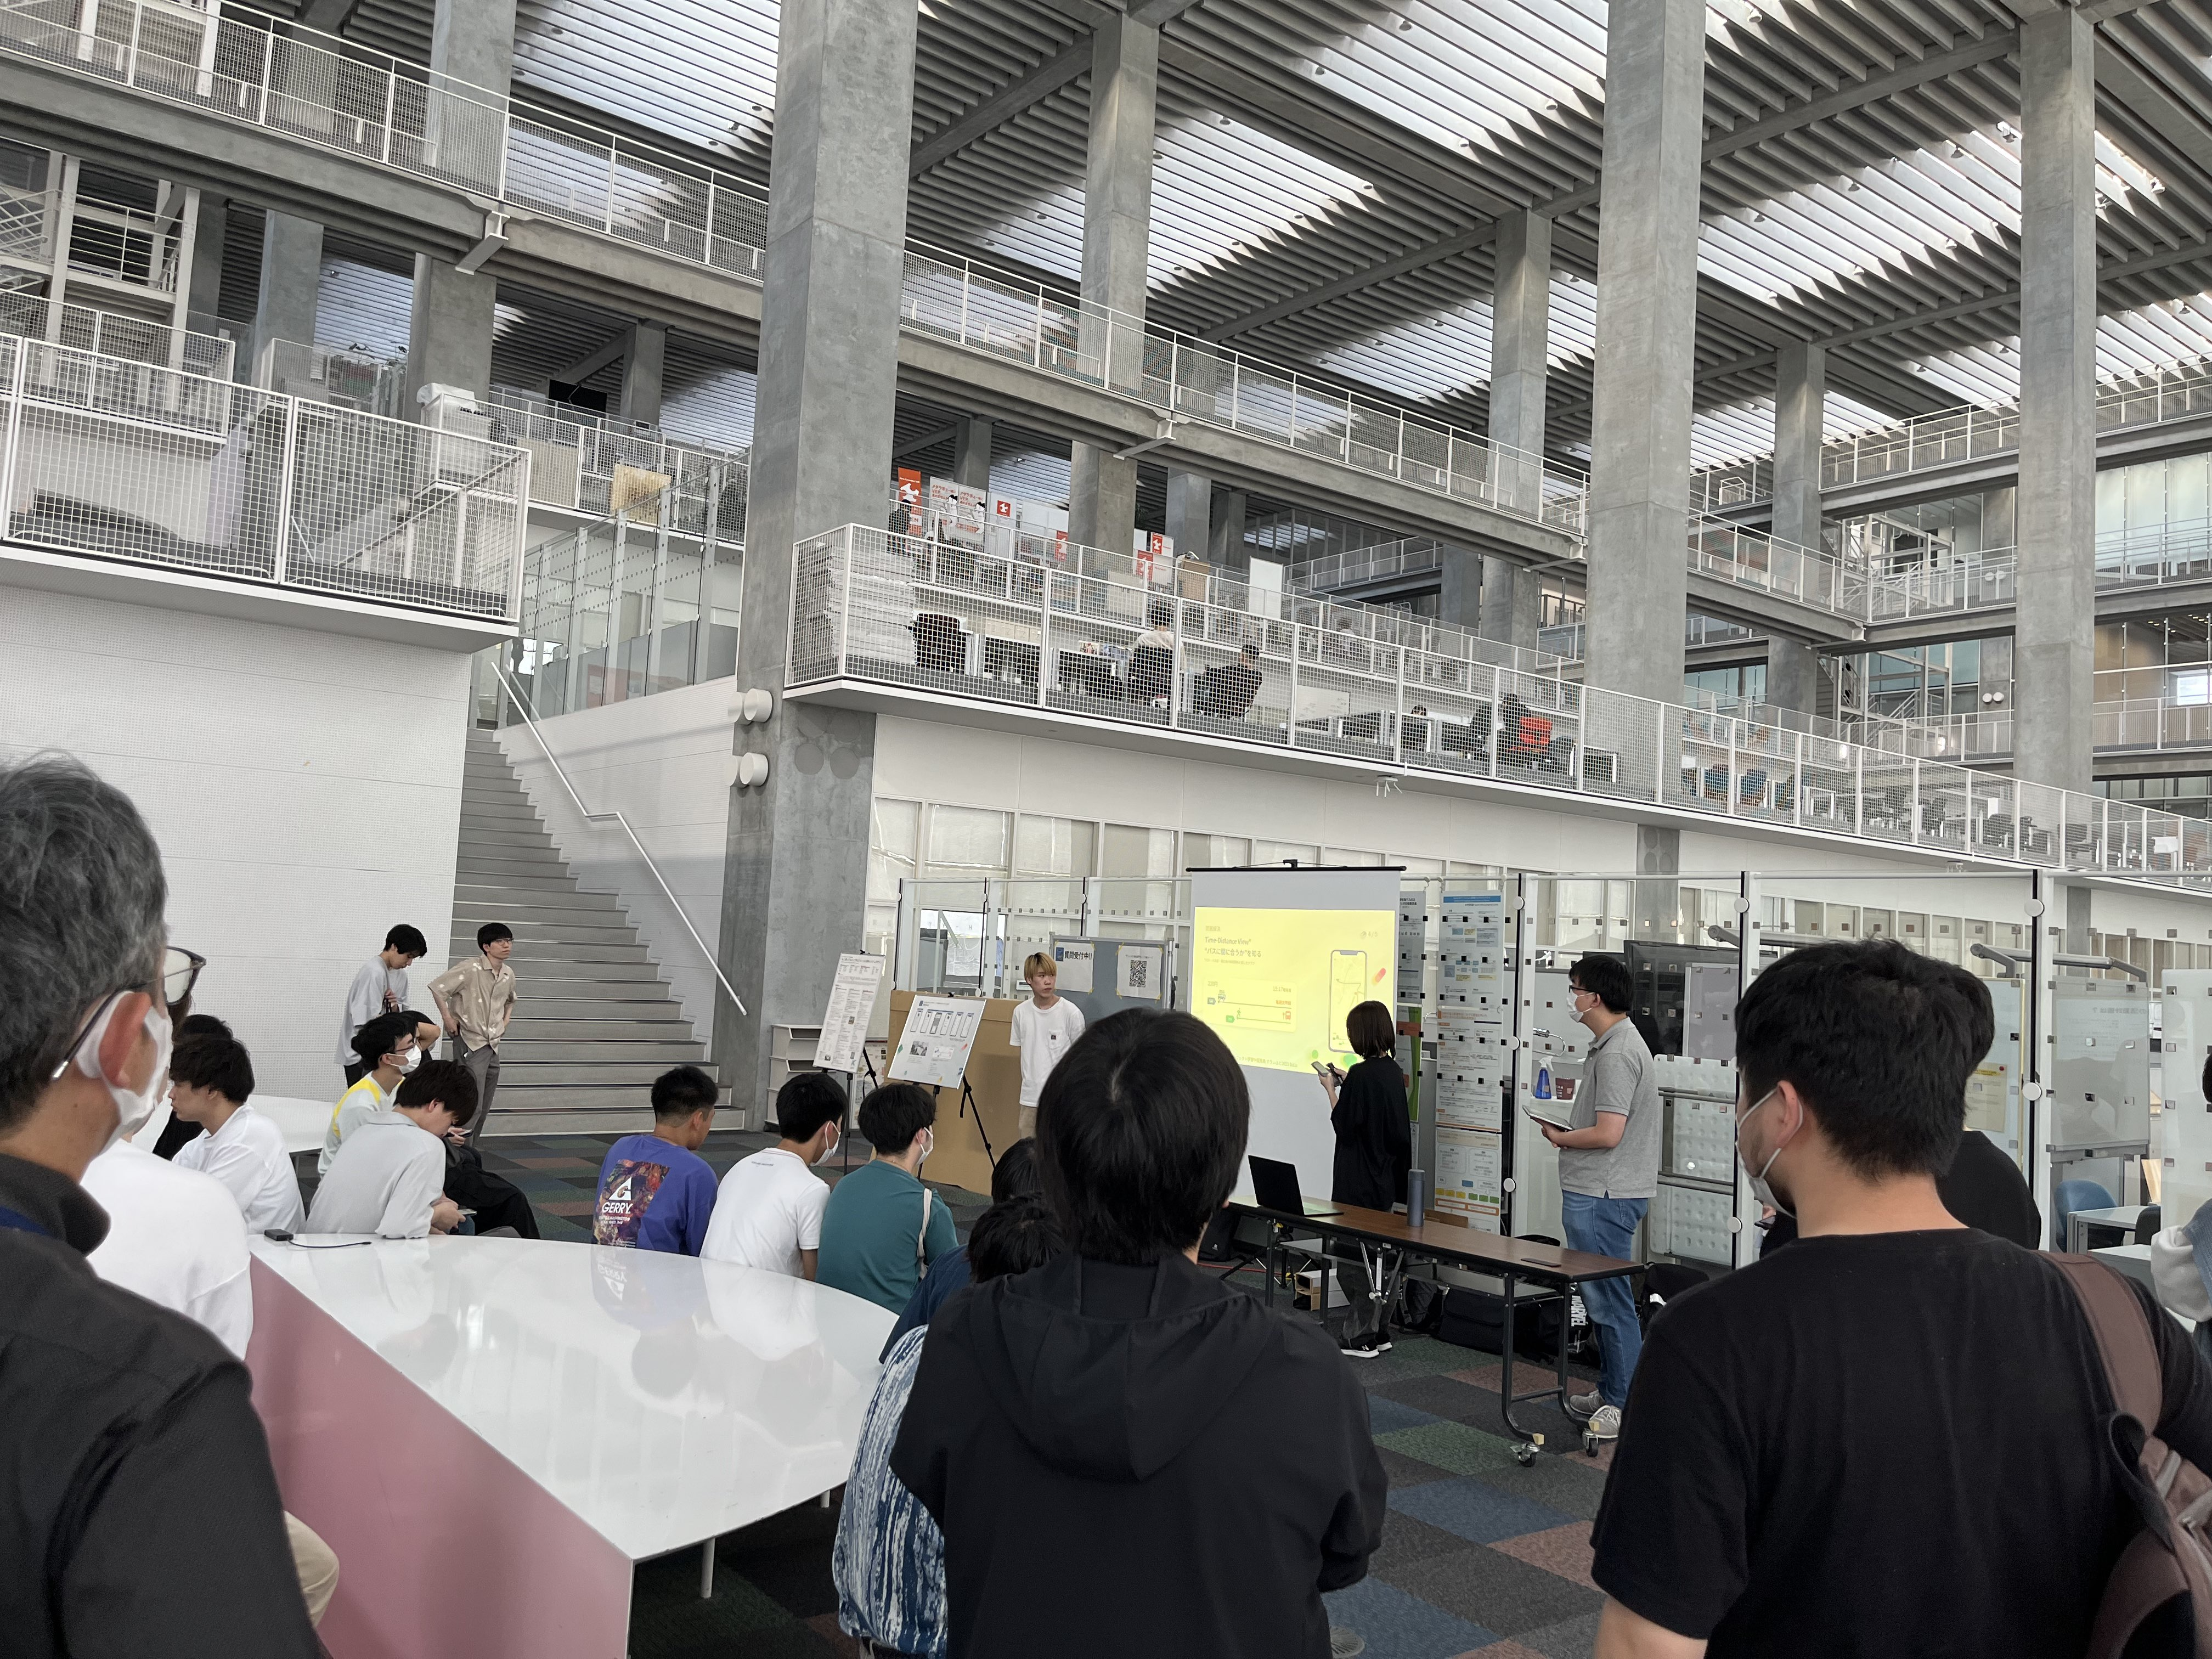
\includegraphics[width=8cm]{images/presen.jpg}
    \caption{中間発表の様子}
    \figlab{tyuukann}
\end{figure}
\bunseki{高橋慧流}

\subsection{フィードバック}
中間発表では，先生方や学生から主にアプリの機能案に関するフィードバックをいただいた．特に，「どこから情報をもってくるのか」という指摘が多くあった．このフィードバックは，アプリの要件定義において重要な視点となり，今後の開発に活かすことができる．また，以下はいただいた具体的なフィードバックである．
\begin{itemize}
      \item HOPEのAPIを使用できるのか
      \item なぜアプリに拘るのか
\end{itemize}
さらに，アイディアとしては以下のものが提案された．
\begin{itemize}
      \item 学生同士の車の相乗り募集
      \item 学生による科目のフィードバック
\end{itemize}

車の相乗りでは特に冬季においてバスが混雑し，相乗りができれば便利だというニーズがある．課題としては，情報の漏れや網羅性の確保が求められる．HOPEの拡張機能でも実現可能ではないかとの提案もあった．科目のフィードバックでは楽単情報やサークル情報，院試情報など，学生間での科目に関する情報共有やフィードバックが重要であるとされた．これらのフィードバックは，アプリのユーザーのニーズや期待に応えるために，フィードバックを踏まえながらアプリの機能や特徴を明確化していきたい．

\bunseki{高橋慧流}

\section{機能の考案}
6月2日にブレインストーミングを用いて考えた．ブレインストーミングでホワイトボードに機能案を書いた（図\ref{fig:kinou}）.その後，その中から学生生活に必要かどうかをメンバーで審議し，必要な機能を絞った．そして機能として大まかに四つの分類に振り分けた．振り分けた内容として，情報発信，情報系，授業系，マップ系とした．情報発信については要らなくなった教科書などを交換するための場を設けることや，教員が不要なった備品を譲渡する場を設けることが挙げられた．情報系は学内で募集しているアルバイト，学内のイベント，講義の過去問，就活の情報がひとまとめに見られることなどが挙げられた．授業系は現在，授業の情報とシラバスが別々のサイトで公開されているため両方を参照するのに当たって相互性を持つようにすること，課題の締め切りを通知，学生から後輩に参考になるような授業のフィードバックアンケートの場を設けるなどが挙げられた．

\begin{figure}[H]
    \centering
    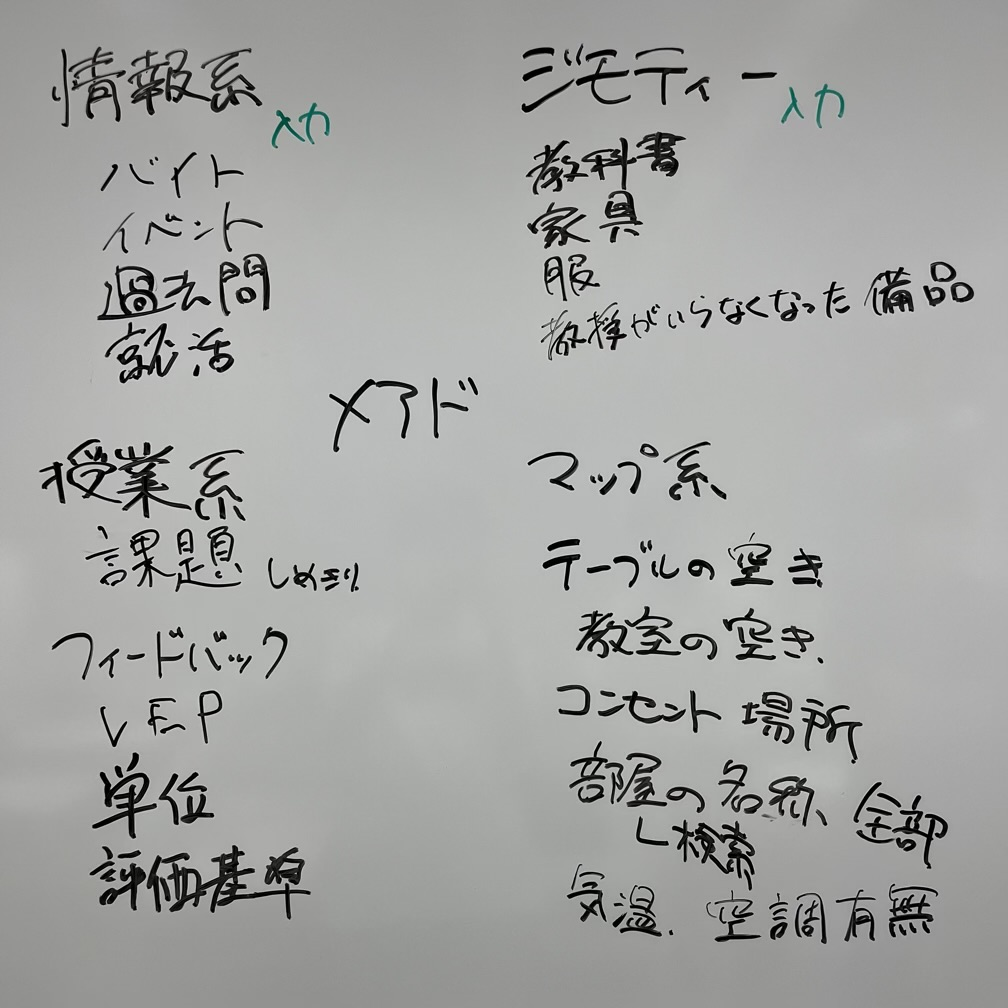
\includegraphics[width=8cm]{images/2_14.jpg}
    \caption{機能の案}
    \figlab{kinou}
\end{figure}
\bunseki{高橋慧流}

\section{プロダクト最終決定}
現時点で，プロダクトバックログの作成を行っていないため，プロダクトの最終決定を行うことはできていない．
\bunseki{鈴木利芳}